\section{Algoritmo}
Al fine di implementare l'algoritmo, si è inialmente pensato di svilupparlo in un ambiente separato dai microservizzi così da avere uno sviluppo più semplificato e di più facile da testare.
Si è quindi utilizzato un ambiente di sviluppo Java con l'ide IntelliJ.

\subsection{brainstorming}
La fase iniziale dell'implementazione è stata affrontata su draw.io dove facendo principalmente riferimento al flowchart ed alla struttura data all'algoritmo sono stati individuati i componenti che si adattassero meglio al nostro pseudocodice. 
L'Output ottenuto da questo brainstorming è infine rappresentato nella seguente immagine:
\begin{figure}[htbp]
	\centering
	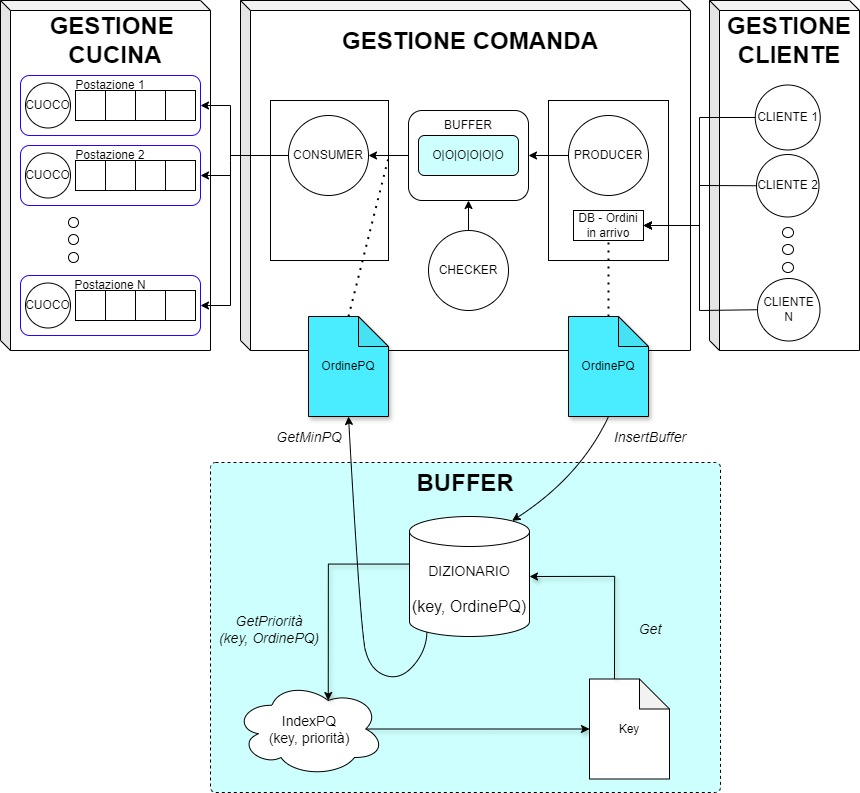
\includegraphics[scale=0.5]{iterazione3/images/Struttura_implementativa_algoritmo.jpg}
	\caption{logico-strutura dell'algoritmo da implementare\label{fig:Struttura_implementativa_algoritmo}}
\end{figure}

\subsection{Adattamento struttura dati}
La scelta implementativa presa ha portato alla ricerca di una struttura equivalente alla \textbf{IndexPriorityQueue}.\\
Dopo una attenta ricerca la struttura scelta è stata la \textbf{IndexMinPQ} \cite{princeton}, basata su una PriorityQueue indicizzata che permette di costuire un heap dove la minima priorità è a radice.
Successivamente, è stata sviluppata una classe \textbf{Dizionario} contenente un dizionario (hashMap) ed un array (ArrayList) di supporto per indicizzare univocamente le chiavi della IndexPriorityQueue ed inoltre mantene riutilizzabili gli stessi indici.\\
Vi era infatti un problema implementativo per il quale ad ogni elemento aggiunto all'heap avrebbe avuto un Id identificativo incrementale causando una esponenzialità di quest'ultimo non desiderata, attraverso il dizionario di supporto è stato quindi possibile riutilizzare degli indici univoci all'interno dell'heap ordinato della indexMinPQ ed avere un accesso diretto all'elemento da estrarre.\\
\begin{figure}[htbp]
	\centering
	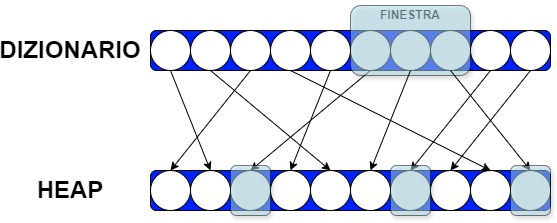
\includegraphics[scale=0.5]{iterazione3/images/dizionario_heap.jpg}
	\caption{associazione dizionario ed heap\label{fig:dizionario_heap}}
\end{figure}

\subsection{Implementazione}
L'effettiva implementazione si è basata su un approccio di sviluppo bottom-up delle varie componenti. \\
Inizialmente è stata sviluppata la struttura dati attraverso i seguenti passaggi:
\begin{itemize}
    \item verificato il corretto funzionamento della IndexMinPQ ed adattato il funzionamento al nostro caso di utilizzo;
    \item implementato il dizionario composto da hashMap e ArrayList associato all'heap della struttura dati;
    \item verificato il corretto funzionamento dell'associazione imposta fra le strutture.
\end{itemize}

Per lo Sviluppo della gestione dei thread:
\begin{itemize}
    \item Si è creato un Buffer semaphore gestito inizialmente da tre thread:
    \begin{itemize}
        \item \textbf{Producer:} verifica la disponibilità di posti all'interno del buffer ed inserisce gli ordini con una priorità iniziale già assegnata in esso;
        \item \textbf{Consumer:} estrae l'elemento con priorità più elevata dalla struttura dati per poi inserirlo all'interno delle code di postazione attraverso una FIFO;
        \item \textbf{Checker:} verifica attraverso una finestra limitata l'aggiornamento di priorità dei vari ordini presenti nel buffer. 
    \end{itemize}
    \item adattato il buffer alle strutture dati utilizzate;
    \item verificato il corretto utilizzo del buffer con le strutture dati con alcuni oggetti test.
\end{itemize}

Infine sono state sviluppate alcune entità e code utili per simulare il percorso degli ordini effettuati dal cliente fino alla coda di postazione designata per ingrediente principale. 
Fra esse abbiamo:
\begin{itemize}
	\item \textbf{Cliente:} ogni cliente rappresenta un thread che genera un ordine;
	\item \textbf{Cuoco:} ogni cuoco rappresenta un thread che riceve degli ordini;
	\item \textbf{Coda postazione:} coda singola che permette di ricevere ordini e processarli come una coda fifo;
	\item \textbf{OrdinePQ:} classe che rappresenta l'ordine e tutti i suoi attributi;
	\item \textbf{Gestione priorità:} classe che permette di gestire i pesi \textbf{p} e \textbf{x} che portano al calcolo del \textbf{valore priorità} di ogni ordine.
\end{itemize}
\newpage
\subsection{Simulazione}
Viene di seguito mostrato un esempio di funzionamento per via dei messaggi di log sulla console
\subsubsection{Setup:}
Per questa simulazione si sono scelti i seguenti valori:
\begin{itemize}
	\item Producer: sleep ogni 500 millisecondi;
	\item Consumer: sleep ogni 2 secondi;
	\item Checker: sleep ogni 3 secondi;
	\item Cliente: 4 thread con sleep random tra 10 e 60 secondi;
	\item Cuoco: 4 thread con sleep in base all'ordine variabile tra 10 e 60 secondi;
	\item Buffer size: 10 posti;
	\item Buffer cucina: 10 posti (numero di ordini totali in cucina);
	\item Capacità singola coda postazione: 5 posti;
	\item 4 Code di postazione: PASTA, RISO, CARNE, PESCE.
\end{itemize}
\subsubsection{Cliente e Producer:}
\begin{figure}[H]
	\centering
	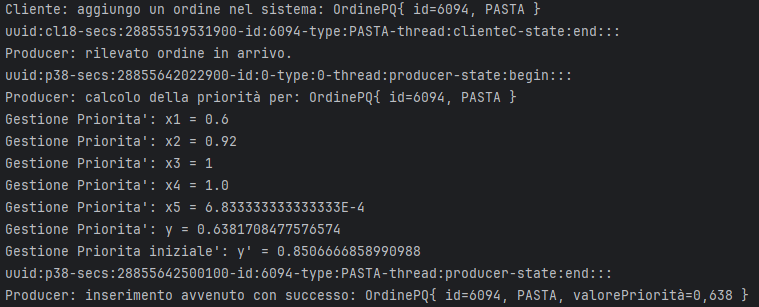
\includegraphics[scale=0.75]{iterazione3/images/Cliente-Producer.png}
	\caption{Funzionamento Thread Cliente e Producer \label{fig:Cliente-Producer}}
\end{figure}
In Figura\vref{fig:Cliente-Producer} è mostrata l'interazione tra il thread Cliente e il Producer, si può notare come il Cliente effettua un'ordinazione aggiungendo un ordine nel sistema, viene mostrato l'id dell'ordine e il tipo di ingrediente principale, successivamente il Producer si attiva e rileva un ordine all'interno della sua coda, prende questo ordine, gli calcola una priorità passando per la classe Gestione Priorità, e lo inserisce nel buffer. Vengono inoltre mostrati sulla console i passi che si compiono per calcolare la priorità. La priorità iniziale $y'$ differisce dalla $y$ poiché è calcolata senza il contributo del parametro $x5$ visto che nullo all'entrata nel buffer (quindi viene calcolata facendo la somma pesata solo dei primi 4 parametri).
\subsubsection{Checker:}
\begin{figure}[H]
	\centering
	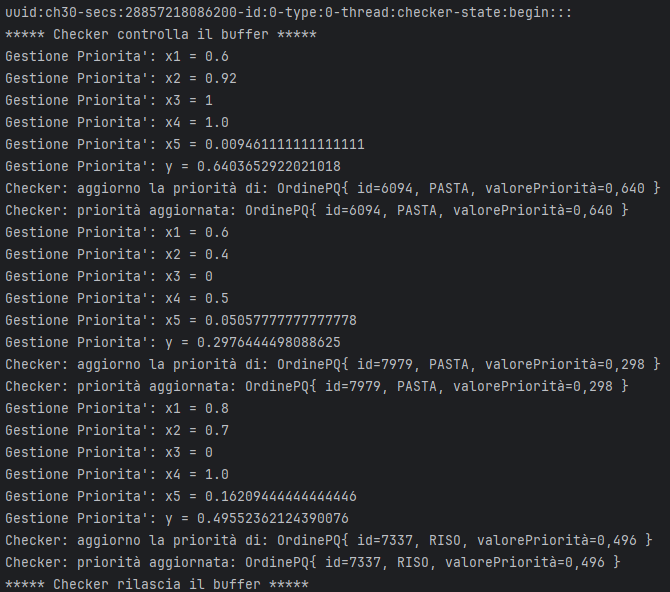
\includegraphics[scale=0.75]{iterazione3/images/Checker.png}
	\caption{Funzionamento Thread Checker \label{fig:Checker}}
\end{figure}
In Figura\vref{fig:Checker} è mostrato il comportamento del Checker, il quale si attiva, controlla in maniera mutualmente esclusiva il buffer e seleziona tramite una finestra mobile gli ordini da controllare ed aggiornare la priorità. Ogni aggiornamento di priorità è seguito da un aggiornamento del buffer im modo da riportare la modifica appena apportata all'ordine.
\subsubsection{Consumer e Producer:}
\begin{figure}[H]
	\centering
	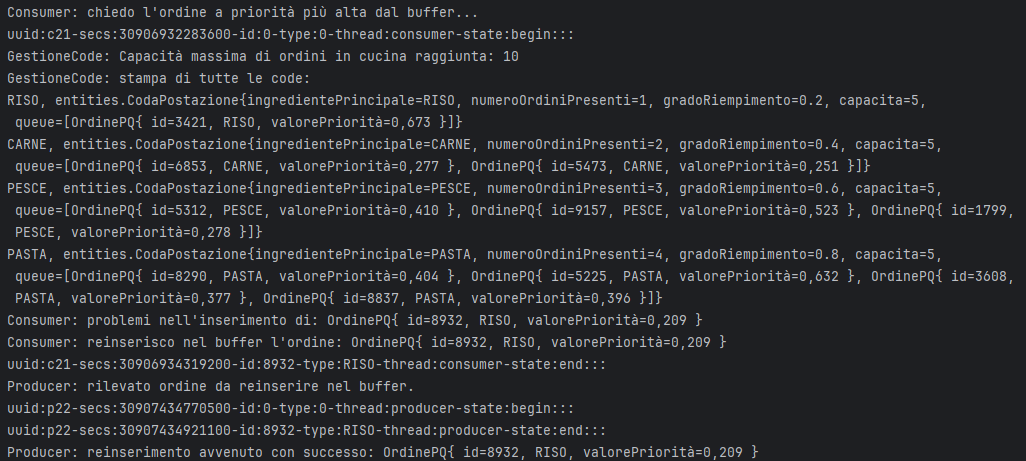
\includegraphics[scale=0.5]{iterazione3/images/consumer-producer.png}
	\caption{Funzionamento Thread Consumer e Producer \label{fig:consumer-producer}}
\end{figure}
In Figura\vref{fig:consumer-producer} è mostrato il caso in cui il Consumer estrae l'ordine a priorità più elevata dal buffer ma non può inviarlo in cucina poiché è stato raggiunto il numero massimo di ordini che possono esistere contemporaneamente in cucina, per questo motivo lo passa al Producer per poterlo reinserire all'interno del buffer. Viene stampato lo stato di ogni coda di postazione per una verifica (infatti si nota che la somma degli ordini in cucina è 10 come segnalato). Il Producer riceve quindi l'ordine e lo reinserisce immediatamente nel buffer.
\subsubsection{Consumer:}
\begin{figure}[H]
	\centering
	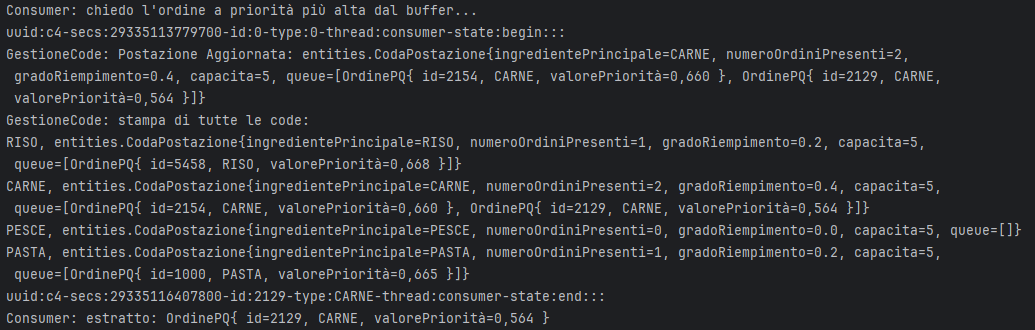
\includegraphics[scale=0.5]{iterazione3/images/Consumer.png}
	\caption{Funzionamento Thread Consumer \label{fig:Consumer}}
\end{figure}
In Figura\vref{fig:Consumer} è mostrato il caso di funzionamento ordinale del Consumer, cioè il caso in cui estrae l'ordine a priorità più elevata dal buffer e lo inserisce nella corrispettiva coda di postazione per ingrediente principale in cucina. Anche in questo caso viene stampato lo stato di ogni coda di postazione per una semplice verifica.
\subsubsection{Cuoco:}
\begin{figure}[H]
	\centering
	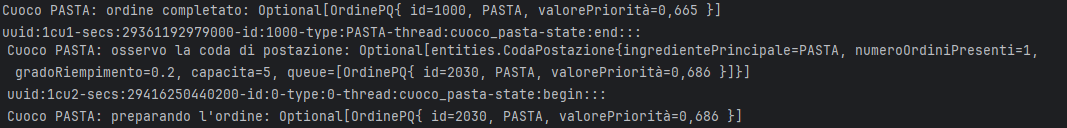
\includegraphics[scale=0.5]{iterazione3/images/Cuoco.png}
	\caption{Funzionamento Thread Cuoco \label{fig:Cuoco}}
\end{figure}
In Figura\vref{fig:Cuoco} è mostro il lavoro del cuoco, nello specifico quello adibito alla postazione dell'ingrediente principale PASTA, il quale finisce di preparare un ordine, invia di conseguenza una notifica di avvenuta preparazione e si mette in attesa sulla propria coda di postazione, rileva quindi un ordine in coda e comincia la preparazione quel nuovo ordine rilevato.
\subsubsection{Dati simulazione:}
Per quanto riguarda i dati della simulazione e l'analisi di questi per valutare la performance dell'algoritmo si fa riferimento alla sezione \vref{sec:analDati}.
\clearpage